\documentclass[a4paper]{tufte-book}
\raggedbottom

%----------%
% SETTINGS %
%----------%

\makeatletter
\def\input@path{{./settings/}}
\makeatother
% settings files
\usepackage{booktabs}

\usepackage{lipsum}
% \usepackage{import}  % for relative paths importing

% Language-related
\usepackage[english]{babel}
\usepackage[autostyle, german=guillemets, english=american]{csquotes}

% Packages
\usepackage{amsmath, mathtools, bm, commath}
\usepackage{physics}
\usepackage{siunitx}
\usepackage{nicematrix}

% General settings
\allowdisplaybreaks     % Allows for equations to break between pages

% Cancel-lines related
\usepackage[thicklines]{cancel}
\renewcommand\CancelColor{\color{xred}}
\newcommand{\cancelcol}[2][xred]{ % This is such a silly solution...
	\renewcommand\CancelColor{\color{#1}}
	\cancel{#2}
	\renewcommand\CancelColor{\color{xred}}
}

% Easier space-notation
\newcommand{\Rs}[1][]{\mathbb{R}^{#1}}
\newcommand{\Cs}[1][]{\mathbb{C}^{#1}}

% Set notation for vectors (currently: bold letters)
\renewcommand{\vec}[1]{\bm{#1}}
\newcommand{\uvec}[1]{\bm{\hat{#1}}}
\newcommand{\vnorm}[1]{\left\| \vec{#1} \right\|}
\newcommand{\cvec}[1]{\bm{\overline{#1}}}
\newcommand{\mat}[1]{\bm{#1}}

% Vector operations
\newcommand{\inner}[2]{\langle #1,#2 \rangle}

% Dual space related
\newcommand{\dualspace}[1]{#1^{*}}
\newcommand{\dualvec}[1]{\vec{#1}^{*}}

% Row- and column-vectors: arguments separated by ";".
% Example: $\vec{a} = \colvec{1;2;3;4}$.
\makeatletter
\newcommand\rcvector[2][\\]{\ensuremath{%
  \global\def\rc@delim{#1}%
    \negthinspace\begin{bmatrix}
      \rc@vector #2;\relax\noexpand\@eolst%
    \end{bmatrix}}}
\def\rc@vector #1;#2\@eolst{%
  \ifx\relax#2\relax
    #1
  \else
    #1\rc@delim
    \rc@vector #2\@eolst%
  \fi}
\makeatother
\newcommand{\colvec}{\rcvector}
\newcommand{\rowvec}[1]{\rcvector[,\;]{#1}}
\newcommand{\GenericRowVec}[2][n]{\rowvec{#2_{1};#2_{2};\dots;#2_{#1}}}
\newcommand{\GenericColVec}[2][n]{\colvec{#2^{1};#2^{2};\vdots;#2^{#1}}}

% Colored vectors
\newcommand{\colorVec}[2]{\color{#1}{\vec{#2}}\color{black}}
\newcommand{\vred}{\colorVec{xdarkred}{v}}
\newcommand{\vblue}{\colorVec{xdarkblue}{v}}
\newcommand{\vgreen}{\colorVec{xdarkgreen}{v}}

% Basis vectors and transformations
\newcommand{\eb}[1]{\vec{e}_{#1}}
\newcommand{\ebc}[1]{\tilde{\vec{e}}_{#1}}
\newcommand{\ebr}[1]{\color{xdarkblue}\eb{#1}\color{black}}
\newcommand{\ebcr}[1]{\color{xdarkred}\ebc{#1}\color{black}}
\newcommand{\oldB}{\color{xdarkblue}B\color{black}}
\newcommand{\newB}{\color{xdarkred}\tilde{B}\color{black}}
\newcommand{\Forw}{\bm{F}}
\newcommand{\Backw}{\bm{F^{-1}}}

% Dark equal?
\newcommand{\beq}{\color{black}{=}}

% Better imaginary unit and natural base notation (to separate from variables)
\newcommand{\iu}{\mathrm{i}\mkern1mu}
\newcommand{\eu}{\mathrm{e}}
\newcommand{\Eu}[1]{\mathrm{e}^{#1}}
\newcommand{\EX}[1]{\exp\left(#1\right)}

% General nice matrix
\newcommand{\GNMatrix}[3]{
  \begin{bNiceMatrix}
    #1_{11} & #1_{12} & \dots & #1_{1#3}\\
    #1_{21} & #1_{22} & \dots & #1_{2#3}\\
    \vdots & \vdots & \Ddots & \vdots\\
    #1_{#21} & #1_{#22} & \dots & #1_{#2#3}
  \end{bNiceMatrix}
}

% Clever references (tufte-latex clashes with \autoref)
% \usepackage{cleveref}
% \crefname{figure}{Figure}{Figure}
% \crefname{equation}{Equation}{Equation}

% Hyperrefs etc.
\usepackage[compatibility=false]{caption}
\usepackage{hyperref}
\hypersetup{
  colorlinks=true,
  linkcolor=blue,
  filecolor=magenta,      
  urlcolor=cyan,
  pdftitle={Spinors for Beginners},
  pdfauthor={Peleg Bar Sapir},
}

% Packages
\usepackage{xcolor}

%%%%%%%%%%%%%%%%%%%%%%%%
%        COLORS        %
%%%%%%%%%%%%%%%%%%%%%%%%

% Normal colors
\definecolor{xred}{HTML}{BD4242}
\definecolor{xblue}{HTML}{4268BD}
\definecolor{xgreen}{HTML}{52B256}
\definecolor{xpurple}{HTML}{7F52B2}
\definecolor{xorange}{HTML}{FD9337}
\definecolor{xdotted}{HTML}{999999}
\definecolor{xgray}{HTML}{777777}
\definecolor{xcyan}{HTML}{80F5DC}
\definecolor{xpink}{HTML}{F690EA}
\definecolor{xgrayblue}{HTML}{49B095}
\definecolor{xgraycyan}{HTML}{5AA1B9}

% Dark colors
\colorlet{xdarkred}{red!85!black}
\colorlet{xdarkblue}{xblue!85!black}
\colorlet{xdarkgreen}{xgreen!85!black}
\colorlet{xdarkpurple}{xpurple!85!black}
\colorlet{xdarkorange}{xorange!85!black}
\colorlet{xdarkcyan}{xcyan!85!black}

% Very dark colors
\colorlet{xverydarkblue}{xblue!50!black}

% Document-specific colors
\colorlet{normaltextcolor}{black}
\colorlet{figtextcolor}{xblue}

% Enumerated colors
\colorlet{xcol0}{black}
\colorlet{xcol1}{xred}
\colorlet{xcol2}{xblue}
\colorlet{xcol3}{xgreen}
\colorlet{xcol4}{xpurple}
\colorlet{xcol5}{xorange}
\colorlet{xcol6}{xcyan}
\colorlet{xcol7}{xpink!75!black}

%%%%%%%%%%%%%%%%%%%%%
%        PGF        %
%%%%%%%%%%%%%%%%%%%%%

\usepackage{pgfplots}
\usepgfplotslibrary{fillbetween}%, colormaps, colorbrewer, patchplots}
\pgfplotsset{
  compat=1.16,
  %% Styles %%
  xyplane/.style = {
    axis x line=middle,
    axis y line=middle,
    xlabel=$x$,
    ylabel=$y$,
    every axis x label/.style={at={(ticklabel* cs:1.02)}, anchor=west},
    every axis y label/.style={at={(ticklabel* cs:1.02)}, anchor=south},
    axis line style={stealth-stealth, very thick, black!65},
    label style={font=\large},
    tick label style={font=\large},
    samples=100,
    xmin=-5, xmax=5,
    ymin=-5, ymax=5,
    grid=both,
    major grid style={black!15},
    minor grid style={black!10},
    xticklabels={,},
    yticklabels={,},
  },
  xynogrid/.style = {
    xyplane,
    major grid style={opacity=0},
    minor grid style={opacity=0},
  },
  xyempty/.style = {
    xyplane,
    axis line style = {draw=none},
    tick style = {draw=none},
    xlabel = {},
    ylabel = {},
    major grid style = {draw=black!0},
  },
  hyperplane1D/.style = {thick, #1},
  %% Function plots
  function/.style = {
    ultra thick, draw=#1,
  },
  filledfunction/.style = {
    function={#1}, opacity=1, fill=#1, fill opacity=0.3,
  },
}

%%%%%%%%%%%%%%%%%%%%%%
%        TikZ        %
%%%%%%%%%%%%%%%%%%%%%%

\usepackage{tikz, tikz-3dplot}
\usetikzlibrary{calc, shapes, intersections, backgrounds, decorations.markings}
\tikzset{
  %% Styles %%
  vector/.style = {#1, ultra thick, -stealth, cap=round},
  pics/ruler/.style n args = {5}{
      code = {
          % Parameters
          \pgfmathsetmacro{\width}{#1}
          \pgfmathsetmacro{\height}{#2}
          \pgfmathsetmacro{\yMaj}{\height/3}
          \pgfmathsetmacro{\yMid}{\yMaj*0.7}
          \pgfmathsetmacro{\yMin}{\yMaj*0.5}
          \pgfmathsetmacro{\dxMaj}{#3}
          \pgfmathsetmacro{\dxMin}{\dxMaj*0.1}
          \pgfmathsetmacro{\maxMajGrad}{ceil((\width-2)/\dxMaj)}
          \pgfmathsetmacro{\maxMidGrad}{\maxMajGrad-0.5}
          \pgfmathsetmacro{\maxMinGrad}{(\maxMajGrad-1)*10}

          % Main rectangle
          \draw[thick, fill=#4] (0,0) rectangle (\width,\height);

          % Graduations
          % Major
          \foreach \x [count=\k from 0] in {1,2,...,\maxMajGrad}
              \draw[thick] ({\x*\dxMaj}, \height) -- ++(0.0,-\yMaj) node[below] (g\k) {$\k$};
          % Middle
          \foreach \y in {1.5,2.5,...,\maxMidGrad}
              \draw[thick] ({\y*\dxMaj}, \height) -- ++(0.0,-\yMid);
          % Minor
          \foreach \z in {1,2,...,\maxMinGrad} 
              \draw[thin] ({\dxMaj+\z*\dxMin}, \height) -- ++(0.0,-\yMin);

          % units label
          \node[below of=g0, font=\small, yshift={11*\height}] {#5};
      }
  },
  arcnode/.style 2 args={                
    decoration={
      raise=#1,             
      markings,   
      mark=at position 0.5 with { 
        \node[inner sep=0] {#2};
      }
    },
    postaction={decorate}
  },
  perpline/.style = {
    very thick, densely dotted, draw=#1
  }
}
\newcommand{\rulerTwoD}[6]{
  \pgfmathsetmacro{\Vx}{#1};
  \pgfmathsetmacro{\Vy}{#2};
  \pgfmathsetmacro{\a}{#3};
  \pgfmathsetmacro{\scale}{3*\a/sqrt(\Vx*\Vx+\Vy*\Vy)};
  \foreach \b in {-#4,...,#4}
    \addplot[very thick, #5] {-(\Vx/\Vy)*x+(\b/\a)};
}

% section numbering
\setcounter{secnumdepth}{2}

% Chapter title
\titleformat{\chapter}
[block]% shape
{\relax\ifthenelse{\NOT\boolean{@tufte@symmetric}}{\begin{fullwidth}}{}}% format applied to label+text
{\itshape\huge\thechapter}% label
{1em}% horizontal separation between label and title body
{\huge\rmfamily\itshape}% before the title body
[\ifthenelse{\NOT\boolean{@tufte@symmetric}}{\end{fullwidth}}{}]% after the title body

\usepackage{enumitem}

% Bold text itemize/enumerate
% Taken from an answer to the TeX StackExchange question #266225
\newenvironment{descitemize}
{\begin{description}[leftmargin=*, before=\let\makelabel\descitemlabel]}
{\end{description}}
\newcommand{\descitemlabel}[1]{\textbullet\ \textbf{#1}:}


%----------%
% DOCUMENT %
%----------%

\begin{document}
% \part{Tests}
% \chapter{General layout test}
% \section{This is a title}\label{sec:title}
\lipsum[2-2]

\begin{marginfigure}
    \begin{center}
    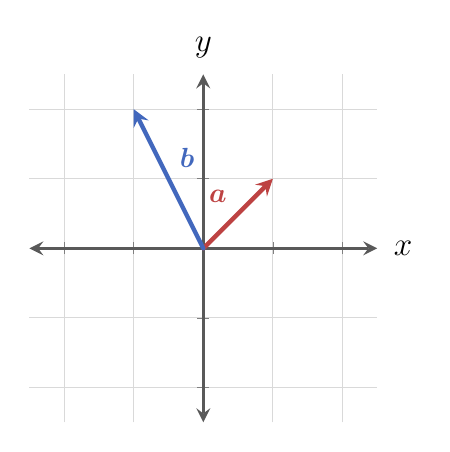
\begin{tikzpicture}
    \begin{axis}[
        xyplane,
        width=6cm, height=6cm,
    ]
        \draw[vector={xred}] (0,0) -- (2,2) node[midway, above left] {$\vec{a}$};
        \draw[vector={xblue}] (0,0) -- (-2,4) node[midway, above right] {$\vec{b}$};
    \end{axis}
    \end{tikzpicture}
    \end{center}
    \caption{A margin figure.}
    \label{fig:margin_figure}
\end{marginfigure}

This is a manualy-typed text. It even points to a figure (see \autoref{fig:margin_figure}).


\makeatletter

%% -- PART 1: Background -- %%
\part{Background Topics}

% Linear algebra
\chapter{Linear Algebra}
\def\input@path{{./parts/background/linear_algebra}}
\section{Preface}
\newthought{The goal of this chapter} is to review a few of the more advanced topics in linear algebra, which are important both for learning the other background topics, as well as the actual topic of spinors.

For example, the topic of dual vectors can help with understanding the what the Dira/bra-ket notation actually means, and cement a deeper understanding of the basic ideas of quantum physics. The topic of absrtact vector spaces provides a good foundation for topics such as geometric- and abstract algebra.

More to be written\ldots

\section{Vectors and Vector Spaces}

\input{linear_transformations}
\input{matrices}
\input{eigenvectors}
\input{quaternions}
\section{Dual Vectors and Dual Spaces}
% Overview:
% Measuring vectors: rulers. How they look like in R2, R3, etc.
% Every ruler can be represented using a specific vector in Rn (direction + density). The measurement is then done via the inner product.
% These inner products actually represent all possible linear functionals Rn->R. They make a linear space on their own.
% Define general idea of dual spaces.
% Basis sets and change of basis - covarience, contravarience and all that.
% relevant SE answers: https://math.stackexchange.com/questions/3749/why-do-we-care-about-dual-spaces

\subsection{Measurements and rulers}
\newthought{Usually, dual vectors are taught} by hitting the students with the definition of a dual space and then analyzing its properties. It's all very abstract and often leaves the students with a constant question in mind: \enquote{why do we care about dual vectors?}

I would like to take a different approach here: instead of confronting you with the definition and then discuss practical details, I will start with explaining \textit{why} we care about dual vectors in the first place.

Let us begin with discussing rulers\sidenote{The idea for this approach comes from a beautiful answer by \textit{Aloizio Macedo} to \href{https://math.stackexchange.com/questions/3749/why-do-we-care-about-dual-space}{a question in the mathematics stack exchange website}.}. A ruler is essentially a geometric object which allows one to measure the \textit{lengths} of different objects by counting the number of graduation lines between the beginning and end of an object (\cref{fig:ruler_measure}). Of course the geometric objects we use normally are vectors.

\begin{figure}
    \begin{center}
        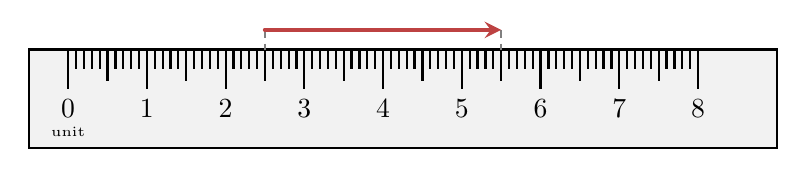
\begin{tikzpicture}
            \draw[thick, fill=black!5] (0.5,0) rectangle (10,1.25);
            \foreach \x [count=\k from 0] in {1,2,...,9} 
                \draw[thick] (\x, 1.25) -- ++(0.0,-0.5) node[below] (g\k) {$\k$};
            \foreach \y in {1.5,2.5,...,8.5} 
                \draw[thick] (\y, 1.25) -- ++(0.0,-0.4);
            \foreach \z in {1.1,1.2,...,8.9} 
                \draw[thick] (\z, 1.25) -- ++(0.0,-0.25);
            \node[below of=g0, font=\tiny, yshift=20] {unit};
            \draw[thick, densely dashed, black!50] (3.5,1.5) -- ++(0,-0.25);
            \draw[thick, densely dashed, black!50] (6.5,1.5) -- ++(0,-0.25);
            \draw[vector={xred}] (3.5,1.5) -- ++(3,0);
        \end{tikzpicture}
    \end{center}
    \caption{Measuring a vector using a ruler: the start of the vector sits at $2.5$ units, while its head is at $5.5$ units. Therefore we say that the vector is $5.5-2.5=3$ units in length.}
    \label{fig:ruler_measure}
\end{figure}

Of course, we can have rulers with different distances between consecutive graduation (i.e. they can be more or less \enquote{dense}), which would yield different measurements for the same vectors. Another property a ruler has its \textit{orientation}: while it is most common to measure by placing a ruler parallel to the distance we wish to measure, it is not \textit{strictly} necessary. If we imagine that the graduation on a ruler are infinitely long and there are infinitely many of them in both directions, we can easily measure vectors that do not align with the ruler (\cref{fig:ruler_measure_at_angle}).

\begin{figure}
    \begin{center}
        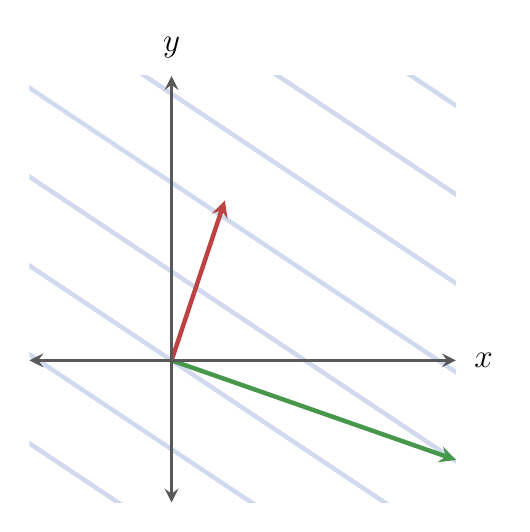
\begin{tikzpicture}
            \begin{axis}[
                xynogrid,
                width=7cm, height=7cm,
                xmin=-2, xmax=4,
                ymin=-2, ymax=4,
                ticks=none,
                axis on top,
            ]
            \pgfmathsetmacro{\Vx}{2};
            \pgfmathsetmacro{\Vy}{3};
            \pgfmathsetmacro{\a}{0.8};
            \pgfmathsetmacro{\scale}{\a/sqrt(\Vx*\Vx+\Vy*\Vy)};
            \foreach \b in {-5,...,5}
                \addplot[ultra thick, xblue!25] {-(\Vx/\Vy)*x+(\b/\a)};
            % \draw[vector={xblue!50!black}] (0,0) -- (\Vx*\scale,\Vy*\scale);
            \draw[vector={xred}] (0,0) -- (0.75,2.25);
            \draw[vector={xdarkgreen}] (0,0) -- (4,-1.4);
            \end{axis}
        \end{tikzpicture}
    \end{center}
    \caption{Measuring two vectors at an angle to the graduation of some ruler. Here the ruler is represented by infinitely long graduations line in blue. Note that although the green vector appears longer than the red vector, it is measured by the ruler to be about $1$ unit long, while the red vector is measured to be a bit more than $2$ units in length.}
    \label{fig:ruler_measure_at_angle}
\end{figure}

\begin{figure}
    \begin{center}
        \tdplotsetmaincoords{70}{110}
        \begin{tikzpicture}[tdplot_main_coords]
            \pgfmathsetmacro{\a}{3}
            \pgfmathsetmacro{\b}{\a+0.5}
            \foreach \z in {-2,-1,...,2}
                \draw[very thick, xblue, fill=xblue, opacity=0.5] (-\a,-\a,\z) -- (-\a,\a,\z) -- (\a,\a,\z) -- (\a,-\a,\z) -- cycle;
            \draw[vector={xdarkblue}] (-\b,\b,-2) -- (-\b,\b,2);
            \draw[vector={xred}] (0,0,-2) -- (\b,0,2);
        \end{tikzpicture}
    \end{center}
    \caption{Measuring two vectors at an angle to the graduation of some ruler. Here the ruler is represented by infinitely long graduations line in blue. Note that although the green vector appears longer than the red vector, it is measured by the ruler to be about $1$ unit long, while the red vector is measured to be a bit more than $2$ units in length.}
    \label{fig:ruler_measure_at_angle}
\end{figure}

\section{The Braket Notation and Einstein's Summation}

\section{Some Formalism and General Vector Spaces}

%% !!! CORRECT ISSUE with \cref and example environment !!! %%

% Outline:
% * Linear algebra on R^n prooved useful (e.g. linear transformations, basis sets, etc.). It would be nice to have similar results for other structures.
% * To find more structures for which we can derive similar ideas, we first need to overview the fundamental properties of vectors in R^n, and see if there are any other structures with similar properties.
% * Fundamental properties
% * Matrices have the same properties! (+elaboration)
% * Polynomial functions have the same properties! (+elaboration)
% * Functions have the same properties! (+elaboration)
% * Using these properties to define a vector space + short discussion.

% \begin{descitemize}
%     \item[Closure of vector addition] the sum of any two vectors $\vec{u}$ and $\vec{v}$ in $\Rs[n]$ is also a vector in $\Rs[n]$ - i.e. 
%     \begin{equation}
%         \text{if}\ \vec{u}+\vec{v}=\vec{w},\ \text{then}\ \vec{w}\in\Rs[n].
%         \label{eq:vector_addition_closure}
%     \end{equation}
%     
%     \item[Commutativity of vector addition] resulting from the parallelogram rule, the addition of vectors is commutative - i.e.
%     \begin{equation}
%         \vec{u}+\vec{v}=\vec{v}+\vec{u}.
%         \label{eq:vector_addition_commutative_2}
%     \end{equation}
%
%     \item[Associativity of vector addition] the order of adding multiple vectors does not matter: for any three vectors $\vec{u},\ \vec{v},\ \vec{w}$ in $\Rs[n]$,
%     \begin{equation}
%         \vec{u}+\left(\vec{v}+\vec{w}\right) = \left(\vec{u}+\vec{v}\right)+\vec{w}.
%         \label{eq:vector_addition_associative}
%     \end{equation}
%     
%     \item[Existence of zero] the zero vector $\vec{0}$ is a neutral to addition - i.e.
%     \begin{equation}
%         \forall \vec{u}\in\Rs[n]:\ \vec{u}+\vec{0}=\vec{0}+\vec{u}=\vec{u}.
%         \label{eq:vector_zero_existence}
%     \end{equation}
%
%     \item[Existence additive inverse] for any vector $\vec{v}\in\Rs[n]$ there's an inverse - i.e
%     \begin{equation}
%         \forall \vec{v}\in\Rs[n]:\ \exists\left(-\vec{v}\right), \vec{v}+\left(-\vec{v}\right) = \vec{0}.
%         \label{eq:vector_zero_addition}
%     \end{equation}
%
%     \item[Closure of scalar multiplication] the result of scaling by $\lambda\in\Rs$ of any vector $\vec{v}\in\Rs[n]$ is also in $\Rs[n]$ - i.e. 
%     \begin{equation}
%         \forall\vec{v}\in\Rs[n] \text{and}\ \forall\lambda\in\Rs:\ \lambda\vec{v}\in\Rs[n].
%         \label{eq:scalar_multiplication_closure}
%     \end{equation}
%
%     \item[Associativity of scalar multiplication] for any two scalars $\lambda,\mu\in\Rs$, the order of scaling a vector $\vec{v}\in\Rs[n]$ doesn't matter - i.e.
%     \begin{equation}
%         \left(\lambda\vec{v}\right)\cdot\mu = \lambda\cdot\left(\mu\vec{v}\right).
%         \label{eq:scalar_multiplication_associative}
%     \end{equation}
%
%     \item[Existnce of unity] the number $1$ is neutral with scaling - i.e.
%         \begin{equation}
%             \forall \vec{v}\in\Rs[n]: 1\vec{v}=\vec{v}.
%             \label{eq:scalar_multiplication_unity}
%         \end{equation}
%
%     \item[Distributive laws] vector addition and scaling are distributive together with addition of scalars, i.e. for any $\vec{v},\vec{u}\in\Rs[n]$ and $\lambda,\mu\in\Rs$:
%         \begin{align}
%             \lambda\left(\vec{v}+\vec{u}\right) &= \lambda\vec{v} + \lambda\vec{u},\ \text{and}\\ \left(\lambda+\mu\right)\vec{v} &= \lambda\vec{v} + \mu\vec{v}.
%             \label{eq:label}
%         \end{align}
% \end{descitemize}

\input{further_reading}

% - Geometric algebra
\chapter{Geometric Algebra}
\def\input@path{{./parts/background/geometric_algebra}}
\section{Preface}
\newthought{The goal of this chapter} is to review a few of the more advanced topics in linear algebra, which are important both for learning the other background topics, as well as the actual topic of spinors.

For example, the topic of dual vectors can help with understanding the what the Dira/bra-ket notation actually means, and cement a deeper understanding of the basic ideas of quantum physics. The topic of absrtact vector spaces provides a good foundation for topics such as geometric- and abstract algebra.

More to be written\ldots


% - Abstract algebra
\chapter{Abstract Algebra}
\def\input@path{{./parts/background/abstract_algebra}}
\section{Preface}
\newthought{The goal of this chapter} is to review a few of the more advanced topics in linear algebra, which are important both for learning the other background topics, as well as the actual topic of spinors.

For example, the topic of dual vectors can help with understanding the what the Dira/bra-ket notation actually means, and cement a deeper understanding of the basic ideas of quantum physics. The topic of absrtact vector spaces provides a good foundation for topics such as geometric- and abstract algebra.

More to be written\ldots


% - Lie groups and algebras
\chapter{Lie Groups and Algebras}
\def\input@path{{./parts/background/lie_groups_algebras}}
\section{Preface}
\newthought{The goal of this chapter} is to review a few of the more advanced topics in linear algebra, which are important both for learning the other background topics, as well as the actual topic of spinors.

For example, the topic of dual vectors can help with understanding the what the Dira/bra-ket notation actually means, and cement a deeper understanding of the basic ideas of quantum physics. The topic of absrtact vector spaces provides a good foundation for topics such as geometric- and abstract algebra.

More to be written\ldots


%% -- PART 2: Spinors -- %%
\part{Spinors}


\makeatother
\end{document}
